%!TEX root = ../../dissertation.tex
%%%%%%%%%%%%%%%%%%%%%%%%%%%%%%%%%%%%%%%%%%%%%%%%%%%%%%%%%%%%%%%%%%%%%%%%%%%%%%%%
\section{Active Measurements and Testbeds}
\label{c6:sec:active-measurements}

Active measurements includes any kind of approach that generates its own network traffic and bases the evaluation on it. Therefore, they are usually conducted on an end-to-end basis, with at lest one side under the control of the experimenter.

Apart from researchers writing their own specialized application for a singular study, active measurements are most often conducted with the help of existing network testbeds, thereby reducing the overall effort. Any new protocol or alterations to existing network protocols are usually best tested in large-scale network testbeds to collect performance data and find side-effects. The presence of background traffic and a large device heterogeneity and diversity are often considered an advantage to a testbed as it better resembles real networks.

Testbeds can be either constructed physically by setting up a number of dedicated machines in a lab or form a virtual overlay spanning over an existing computer network. Both of these principles work well for wired networks and there are a lot of examples of successful testbeds constructed with these principles. Currently one of the largest installations is PlanetLab~\cite{chun2003planetlab}, consisting of dedicated machines located at a number of University sites. An experimenter can instantiate a \textit{slice} --- a portion of the overlay network made up of number of interconnected \glspl{VM} hosted on the various machines --- and conduct her studies. Thus, many experiments can run concurrently.

Several testbeds devote themselves to wireless and mobile networks. These are usually either assembled in a closed laboratory environment, SmartLab\footnote{\url{http://smartlab.cs.ucy.ac.cy/}} or EmuLab\footnote{\url{http://www.emulab.net/}} come to mind, or hand out subsidized mobile devices prepared with custom firmwares to volunteers which need to allow running network experiments on them. The approach is taken, e.g., by NetSense~\cite{Striegel:2013:LLN:2491159.2491171} and PhoneLab\footnote{\url{https://www.phone-lab.org/}}~\cite{Nandugudi:2013:PLP:2536714.2536718}. The latter approach raises some interesting issues concerning the volunteers' privacy which will be covered in the next section.

All of these testbeds consist of rather uniform nodes and access to it requires some amount of manual administrative effort. Other testbeds take an alternative route on these issues, for example the Seattle Testbed\footnote{\url{https://seattle.poly.edu/html/}}~\cite{Cappos:2009:SPE:1508865.1508905}. Its overlay network comprises of small software sandboxes installable on a wide range of device types. Experimenters gain automatic access to a portion of the overlay through a clearing house and are resource-restricted to their slice by a hypervisor. As Seattle is available to both conventional desktop and server computers as well as Android smartphones, the overlay composition very heterogeneous. Therefore, the node stability and availability can vary substantially over time, caused amongst other things by the individual uptime of the computers following typical diurnal cycles and mobility-related connectivity issues. While this results in a more realistic picture of a network, it simultaneously makes the execution of the actual study more difficult as these churning issues have to be dealt with.

The requirements specific to conducting reliable streaming experiments are low. As usually a fully pull-based approach is utilized, full control over the server containing the streaming files is not necessary. It is also generally not required to display the actual video on the client in reliable streaming as it always will be a pixel-perfect representation any way. Therefore, the buffer-emulation measurement approach presented in Section~\ref{c3:sec:measurements} can be employed here. The measurement devices only have to record the transmission traces of the streaming process and make them available to the emulation process. The latter can for example also be performed in a centralized and asynchronous matter as long as only non-adaptive streaming is measured.


%%%%%%%%%%%%%%%%%%%%%%%%%%%%%%%%%%%%%%%%%%%%%%%%%%%%%%%%%%%%%%%%%%%%%%%%%%%%%%%%
\subsection{Enriching Mobile Measurements with Additional Metadata}
\label{c6:sec:sensorium}

While transmission traces might be the bare minimum to conduct reliable streaming measurements, meaningful mobile measurement can include much more metadata, giving insightful indication of the device's current state.

Mobile devices have access to a vast array of data. On the one hand does the networking stack itself contain much information on its state, as discussed in the previous chapter. The current radio and mobility state is especially relevant to mobile streaming measurements as it directly influences the link's \gls{QoS} parameters. 

But modern mobile devices additionally contain an ever-growing number of sensors, including \gls{GPS}, accelerometers, temperature, pressure, luminosity, humidity, fingerprint, heartbeat, and several cameras and microphones. Moreover, further radio interfaces (WiFi, Bluetooth, \acrshort{NFC}) gather data on network availability and signal quality. Each additional data source can help in quantifying the physical position, orientation and state of the device and even quantify the ``state'' of its user. Even the NSA is allegedly more interested in metadata in general than actual data for this reason.\footnote{\url{http://www.wired.com/2013/06/phew-it-was-just-metadata-not-think-again/}}

Active measurements in mobile networks should make use of metadata and correlate it to the regular measurement data to achieve a finer result granularity. Alternatively, sensor data can also be used for new kinds of evaluations. Questions like ``Can this device stream watch video at a satisfactory quality at certain locations?'' can be raised and answered.


%%
\subsubsection{Metadata and Privacy}

While the actual experiment usually runs in a strict sandbox environment with no access to actual data on the device, allowing sensor and metadata access intentionally creates holes in this isolation model. As informative metadata can be for network studies as intrusive is unmediated access to this data for the device's user.

In a pure lab environment this poses no problem as there will be no device owner whose information can be leaked. However, preserving the privacy of actual device users running network testbed software is absolutely critical for a number of reasons:

\begin{itemize}

	\item For ethical reasons as stated in several ethics proclamations, for example in the well-known hacker ethics\footnote{\url{http://www.ccc.de/hackerethics}} which states to \textit{``Use public data, protect private data.''}. This is often called the principle of data economy and minimalization, aiming to prevent abuse and minimize the effects of accidental data leakage.

	\item User acceptance is a very important aspect. Testbeds need to have a sufficiently large installation base to achieve meaningful results. But users might choose not to participate if the testbed application is too intrusive. There needs to be a balance between revealing and protecting privacy sensitive data. The acceptance can also be increased by information and disclosing employed data. This servers the additional purpose of educating the user of privacy sensitive data.

	\item Lastly, there are legal constraints to consider when dealing with personal information. In Germany, for example, several fundamental constitutional rights restrict the use of personal data. These are the \textit{``Recht auf informationelle Selbstbestimmung''}\footnote{\url{https://www.bmi.bund.de/DE/Themen/Gesellschaft-Verfassung/Datenschutz/Informationelle-Selbstbestimmung/informationelle-selbstbestimmung_node.html}} and the \textit{``Grundrecht auf Gewährleistung der Vertraulichkeit und Integrität informationstechnischer Systeme''}\footnote{\url{https://www.bundesverfassungsgericht.de/entscheidungen/rs20080227_1bvr037007.html}}.

\end{itemize}

To conclude, network measurement testbeds have to regulate, filter, adjust, or outright prevent access to sensitive data. Existing testbeds usually do not take a technical but rather a bureaucratic approach to this problem. For example, all experiments in the aforementioned PhoneLab require approval from a review board.

But that does not mean that there are no technical means available. Looking outside of the field of network testbeds, some research and even usable implementations are available. 

A very basic and static approach to protecting privacy data is implemented in the regular versions of both iOS and Android. During installation any application has to request specific rights for each sensor source to be able to use it in the future. The ``Privacy Guard'' feature\footnote{\url{https://plus.google.com/+CyanogenMod/posts/gk7X3HjNvnH}} in the custom Android firmware CyanogenMod\footnote{\url{http://cyanogenmod.org/}} provides the additional capability to monitor and revoke any sensor permissions at runtime. Other approaches include increasing the sensor permission granularity~\cite{Jeon:2012:DAM:2381934.2381938} or tagging sensor data at the source to better track and find privacy leaks in applications~\cite{enck2010taintdroid}.


%%
\subsubsection{Sensorium Framework}

Even with these approaches at hand, the privacy issue should be mitigated further beyond the binary allow/deny access approach. Also, it usually is a complicated task for experimenters to access all the various sensors,each answering to a different \gls{API}. \textit{Sensorium}~\cite{raf2013sensorium} was created during the course of this thesis to remedy both of these issues. Sensorium is a generic unified sensor reading framework that interfaces with other applications as well as network nodes and provides the sensor readout to them. More importantly, a fine-grained multi-level privacy control model is implemented.


%%
\paragraph{Architecture}

\begin{figure}[htb]
	\centering
	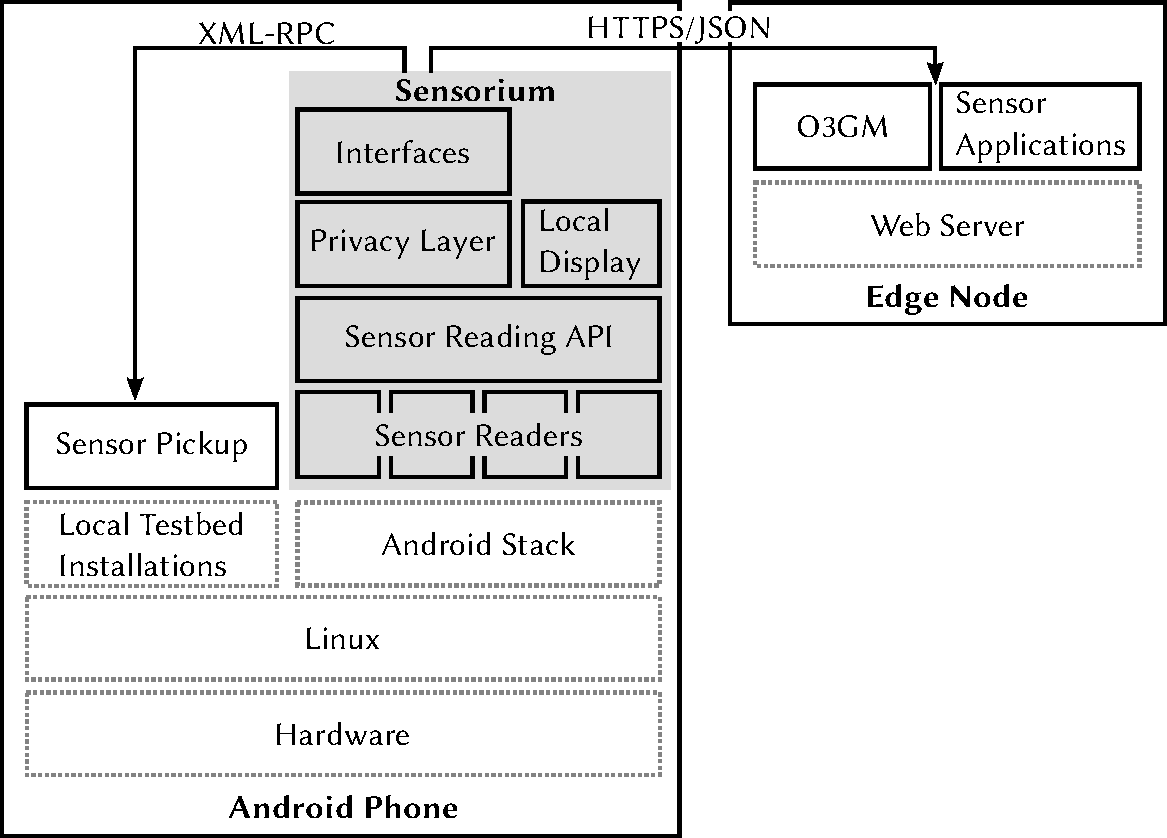
\includegraphics[width=0.8\textwidth]{images/sensorium-arch.pdf}
	\caption{Sensorium architecture interfacing with other applications. Previously existing components are marked with a dotted line.}
\label{c5:fig:architecture}
\end{figure}

Figure~\ref{c5:fig:architecture} overviews the components of Sensorium's architecture. The individual sensor drivers are placed on top of the operating system and take care of reading sensor values from platform-specific interfaces and pushing them upwards into a common registry to be read by the sensor reading \acrshort{API}. All sensor data is relayed both to a local display as well as to all outbound interfaces. Due to the layered architecture, contributors can simply extend or substitute the existing layers. New drivers or additional outbound interfaces can be easily implemented in this way. 

The existing outbound interfaces include an \gls{HTTPS} client that pushes \acrshort{JSON} data to any active network experiment server where the data can be further processed. To connect to programs running locally on the same device, the \acrshort{XML}-\acrshort{RPC} interface can be polled. Pull-based access from sources other than the local host is not allowed for security reasons. However, any data leaving Sensorium must first pass through the privacy layer, which filters the data based on the user's preferences.


%%
\paragraph{Privacy Model}

This privacy layer allows for a fine-grained control over the amount and precision of data that the system is sharing. A settings \acrshort{GUI} provides the user full control over her privacy. Here, she can choose the amount of information she is willing to reveal for each sensor. Based on this preference, the privacy layer then either outright prevents access to specific values or reduces their impact by anonymizing them.

This anonymization task can work in several levels. Apart from completely replacing it with a running number, the value could also be hashed. In many cases context-sensitive anonymization approaches are available. For example, the precision of a geo-location could simply be reduced down to a city-level or even country-level.

As the user is always in firm control of the process, she should be more accepting of actual network experiments that use this kind of data. However, such studies need also cope with the fact that they might get incomplete or partially anonymized data.


%%
\paragraph{Implementation}

\begin{figure}[htb]
	\centering
	\begin{subfigure}[b]{0.45\textwidth}
		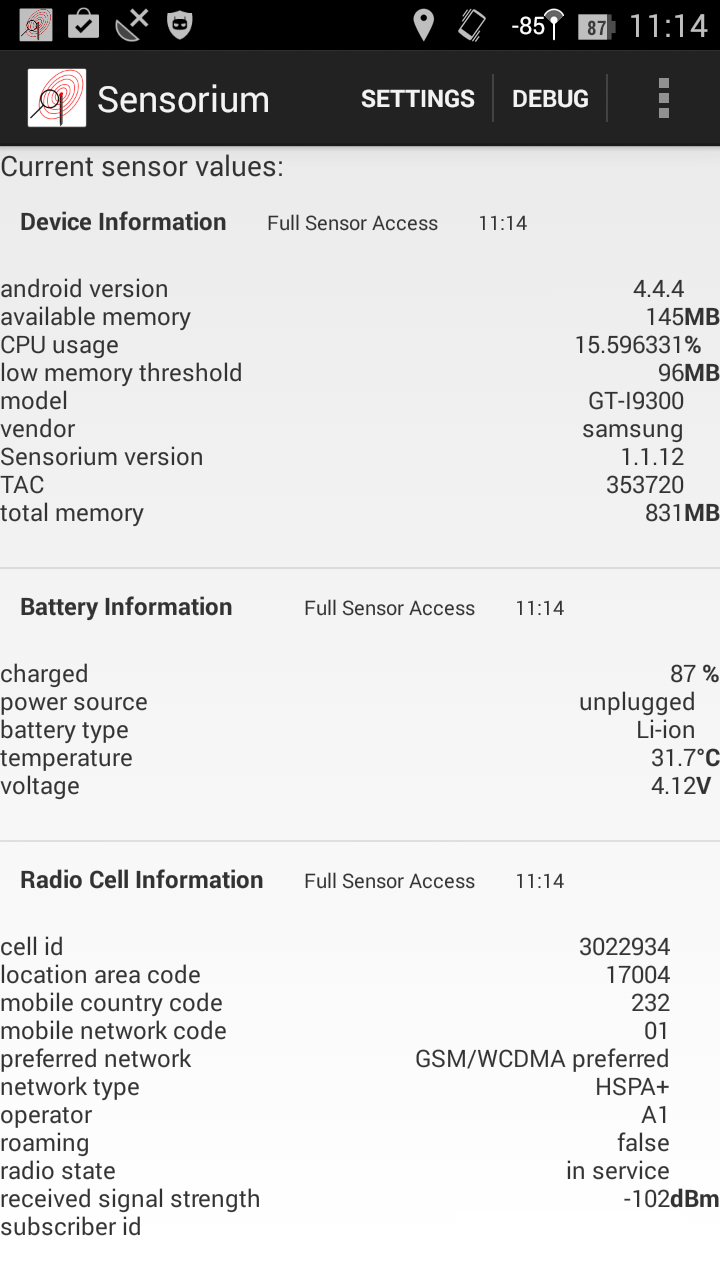
\includegraphics[width=\textwidth]{images/sensorium.png}
		%\caption{Stalling occurs without handover hinting.}
		%\label{c5:fig:streaming-hinting-no-cl}
	\end{subfigure}%
	\hfill
	\begin{subfigure}[b]{0.45\textwidth}
		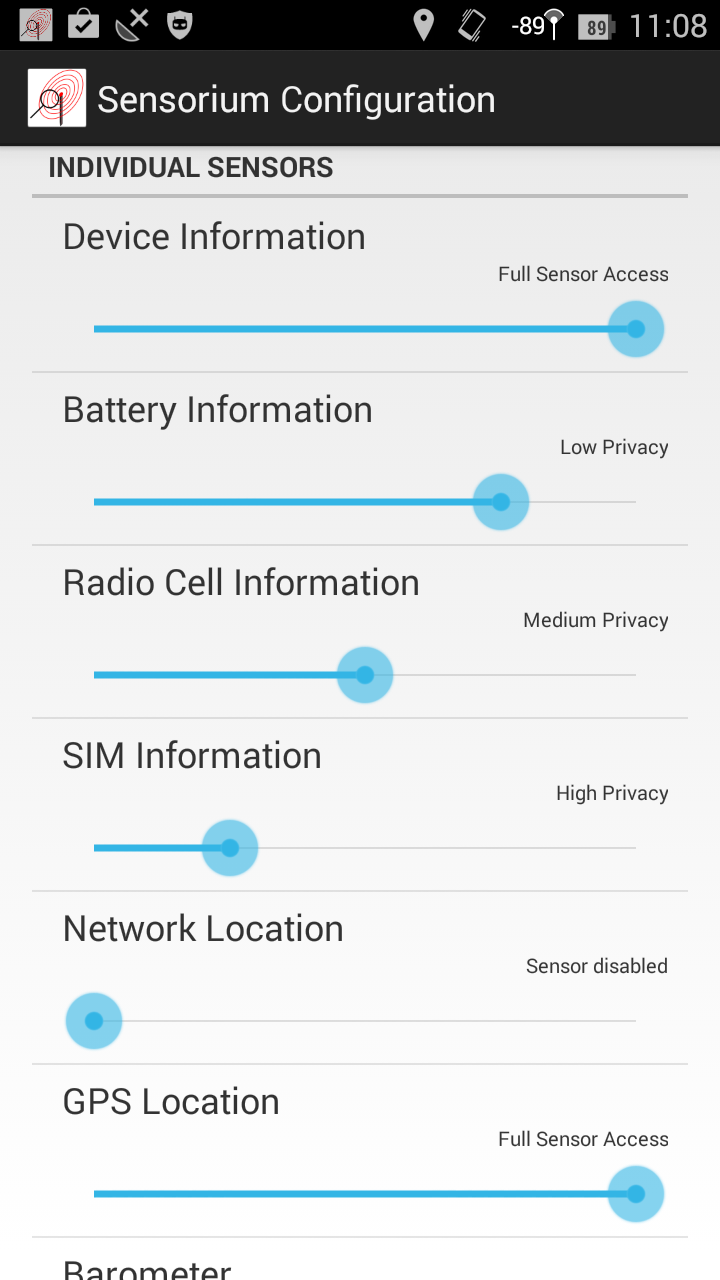
\includegraphics[width=\textwidth]{images/sensorium-settings.png}
		%\caption{Stalling can be prevented by hinting and proactively filling the playback buffer.}
		%\label{c5:fig:streaming-hinting-cl}
	\end{subfigure}%
	\caption{Sensorium sensor values display and settings screenshots.}
\label{c5:fig:sensorium}
\end{figure}

Sensorium is currently targeted at and implemented on the Android platform.\footnote{More information is available at \url{https://github.com/fmetzger/android-sensorium}.} It can be installed on any Android without any modification. Screenshots of the sensor display and settings menu of the application are depicted in Figure~\ref{c5:fig:sensorium}. Drivers for most of the typically available sensors are implemented.

Sensorium was demoed at the NetSys 2013 conference and has since then been available in various app stores. Data from the Google Play Store suggests at least \numprint{50} concurrently running device installations across several countries, carriers and device types. Albeit a still low number, as there was no real advertisement conducted, this could indicate its feasibility as a companion application to a network testbed. Of note are also two related applications that intend to follow up on Sensorium's approach in the future: The Sensibility Testbed\footnote{\url{https://sensibilitytestbed.com/}}, which tightly couples itself to the aforementioned Seattle platform, and BlurSense\footnote{\url{https://blursense.poly.edu/}}~\cite{6798970}, aiming to improve the sensor value anonymization efforts. 


%%
\paragraph{Sensorium Usage}

Sensorium was originally written for two specific targets. First, it was intended as a prototype sensor extension to the Seattle testbed. Pre-anonymized data was to be delivered through the \acrshort{XML}-\acrshort{RPC} interface to a locally running Seattle installation. Any experiment running in this sandbox could then facilitate this sensor data.

\begin{figure}[htb]
	\centering
	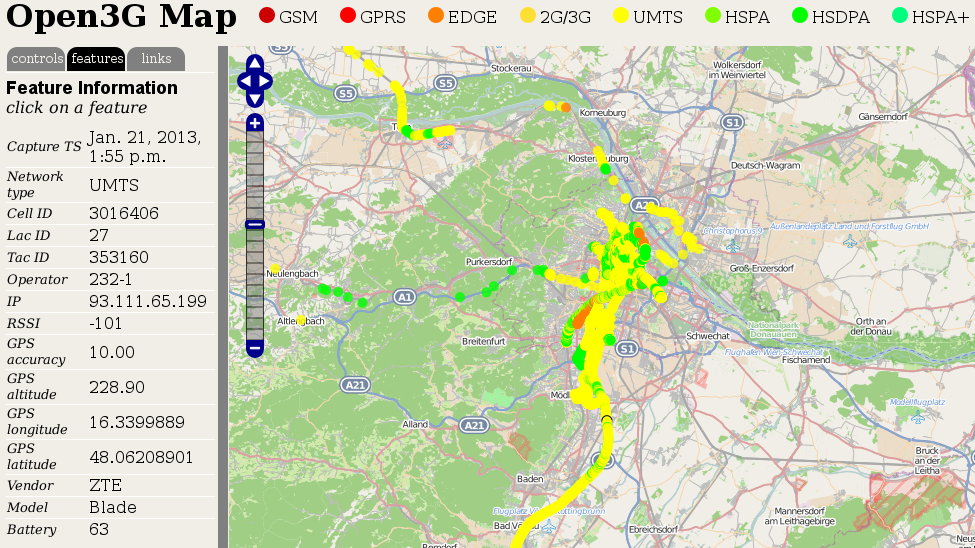
\includegraphics[width=\textwidth]{images/o3gm.png}
	\caption{The \acrshort{O3GM} web page, displaying a \acrshort{3G} coverage measurements layer with data collected by Sensorium on top of the OpenStreetMap base layer.}
\label{c5:fig:ogggm}
\end{figure}

Second, to present what actually can be done with smartphone sensing data, \gls{O3GM}\footnote{\url{https://o3gm.cs.univie.ac.at/o3gm/}}\footnote{\url{https://github.com/lukpueh/Open3GMap}} was created, which visualizes mobile coverage data. \gls{O3GM} is a Web service, that makes use of Sensorium's \acrshort{JSON} upload feature, displaying geo-located \gls{3G} radio access quality information in an OpenStreetMap overlay (using OpenLayers\footnote{\url{http://openlayers.org/}}) as can be seen in Figure~\ref{c5:fig:ogggm}

Coverage data is usually only available to mobile operators, which have not interest to share this information. Other projects such as OpenSignalMaps\footnote{\url{http://opensignal.com/}} and Sensorly\footnote{\url{http://www.sensorly.com/}}, as well as corporations like Google and Apple collect these data, but are very restrictive regarding usage by third parties. \gls{O3GM} data is freely available under an open content license.

Coverage data can again also be helpful to determine the viability of mobile reliable streaming. For example, knowing the \gls{RAT} and signal strength of a specific path can help make informed decisions on which stream quality to choose at which time for adaptive streaming. If Sensorium would be combined with the reliable streaming measurement framework of Section~\ref{c3:sec:measurements}, one could check rather easily for correlations between stalling phases and mobility events.


%Improving wireless network performance using sensor hints \cite{ravindranath2011improving}


% HomeLab: A Platform For Conducting Experiments With Connected Devices In The Home \cite{Singh:2013:HPC:2486001.2491701}
% authentication-based privacy, fully up to the experimenter

% phonelab privacy approach:
% Large (288 devices) smartphone testbed
% each participant can choose to participate in individual experiments
% open for experimenters upon approval, centralized experiment execution by the review board
% privacy guaranteed only through the project review board, not through technical means (centralized, not distributed)
% bureaucratic apprach to experimentation and privacy, not automatized
% relies on Androids privacy mechanisms (imho: do not work for this type of project)
% real people (as opposed to emulab, planetlab,...)!
% interesting study for wifi->3g vertical handover locations -> could extend wifi coverage studies and wifi planning

%http://campar.in.tum.de/Chair/KalmanFilter
%https://dsp.stackexchange.com/questions/320/is-a-kalman-filter-suitable-to-filter-projected-points-positions-given-euler-an/321\#321
%``Sensor Fusion''?

%https://guardianproject.info/

% NativeWrap \url{http://research.csc.ncsu.edu/security/nativewrap} \cite{Nadkarni:2014:NAH:2627393.2627412}
% Use website as app instead of native app, thus reducing permissions


% Sensorium play store stats:
% usage peak: 51 concurrent device installs August 2014
% total installs: 475 as of august 2014
% on various types of devices (including tablets)
% across several countries (top: US, DE, AT, India, Turkey)
% and all carriers
% with not particular advertisement (demo presentation at one national conference NetSys 2013)

